%package list
\documentclass{article}
\usepackage[top=3cm, bottom=3cm, outer=3cm, inner=3cm]{geometry}
\usepackage{graphicx}
\usepackage{url}
%\usepackage{cite}
\usepackage{hyperref}
\usepackage{array}
\usepackage{multicol}
\newcolumntype{x}[1]{>{\centering\arraybackslash\hspace{0pt}}p{#1}}
\usepackage{natbib}
\usepackage{pdfpages}
\usepackage{multirow}
\usepackage{float}
\usepackage[normalem]{ulem}
\useunder{\uline}{\ul}{}




%%%%%%%%%%%%%%%%%%%%%%%%%%%%%%%%%%%%%%%%%%%%%%%%%%%%%%%%%%%%%%%%%%%%%%%%%%%%
%%%%%%%%%%%%%%%%%%%%%%%%%%%%%%%%%%%%%%%%%%%%%%%%%%%%%%%%%%%%%%%%%%%%%%%%%%%%
\newcommand{\csemail}{vmachacaa@unsa.edu.pe}
\newcommand{\csdocente}{Vicente Machaca Arceda}
\newcommand{\cscurso}{Algoritmos y Estructura de Datos}
\newcommand{\csuniversidad}{Universidad Nacional de San Agustín}
\newcommand{\csescuela}{Maestría en Ciencia de la Computación}
\newcommand{\cspracnr}{01}
\newcommand{\cstema}{--}
%%%%%%%%%%%%%%%%%%%%%%%%%%%%%%%%%%%%%%%%%%%%%%%%%%%%%%%%%%%%%%%%%%%%%%%%%%%%
%%%%%%%%%%%%%%%%%%%%%%%%%%%%%%%%%%%%%%%%%%%%%%%%%%%%%%%%%%%%%%%%%%%%%%%%%%%%


\usepackage[english,spanish]{babel}
\usepackage[utf8]{inputenc}
\AtBeginDocument{\selectlanguage{spanish}}
\renewcommand{\figurename}{Figura}
\renewcommand{\refname}{Referencias}
\renewcommand{\tablename}{Tabla} %esto no funciona cuando se usa babel
\AtBeginDocument{%
	\renewcommand\tablename{Tabla}
}

\usepackage{fancyhdr}
\pagestyle{fancy}
\fancyhf{}
\setlength{\headheight}{30pt}
\renewcommand{\headrulewidth}{1pt}
\renewcommand{\footrulewidth}{1pt}
\fancyhead[L]{\raisebox{-0.2\height}{
\includegraphics[width=3cm]{img/logo_unsa}}}
\fancyhead[C]{}
\fancyhead[R]{\fontsize{7}{7}\selectfont	\csuniversidad \\ \csescuela \\ \textbf{\cscurso} }
\fancyfoot[L]{MSc. Vicente Machaca}
\fancyfoot[C]{\cscurso}
\fancyfoot[R]{Página \thepage}







\begin{document}
	
	\vspace*{10px}
	
	\begin{center}	
		\fontsize{17}{17} \textbf{ Práctica \cspracnr}
	\end{center}
	%\centerline{\textbf{\underline{\Large Título: Informe de revisión del estado del arte}}}
	%\vspace*{0.5cm}
	

	\begin{table}[h]
		\begin{tabular}{|x{4.7cm}|x{4.8cm}|x{4.8cm}|}
			\hline 
			\textbf{DOCENTE} & \textbf{CARRERA}  & \textbf{CURSO}   \\
			\hline 
			\csdocente & \csescuela & \cscurso    \\
			\hline 
		\end{tabular}
	\end{table}	
	
	
	\begin{table}[h]
		\begin{tabular}{|x{4.7cm}|x{4.8cm}|x{4.8cm}|}
			\hline 
			\textbf{PRÁCTICA} & \textbf{TEMA}  & \textbf{DURACIÓN}   \\
			\hline 
			\cspracnr & Algoritmos de ordenamiento  & 3 horas   \\
			\hline 
		\end{tabular}
	\end{table}
	
	
	\section{Datos de los estudiantes}
	Grupo: N° 8
	\begin{itemize}
		\item Integrantes: 
		\begin{itemize}
			\item Esai Josue Huaman Meza
			\item Alan Jerry Reyes Robles
			\item Jorge Luis Zegarra Guardamino
			\item Nestor Giraldo Calcinas Huaranga
		\end{itemize}		
	\end{itemize}
	
	
	
	
	
	
	\section{Introducción}
	
	Se hara un análisis comparativo 04 algoritmos de ordenamiento, buscando estudiar la complejidad de cada uno de estos y como las diferentes formas de resolver un mismo problema pueden afectar los tiempos de ejecución.
	
	Dado que para hacer un buen análisis se deben correr muchas pruebas, cree un par de scripts que me permitieran automatizarlas de forma tal que se pudieran correr de forma continua sin intervención. Se procura crear un pequeño ambiente controlado por lo que se usara una sola PC para reallizar las pruebas donde no estuvieran ejecutandose en paralelo otras tareas, dado que los tiempos de ejecución de cada prueba puede verse afectado al estar compartiendo recursos con otros procesos.

    En cada máquina se corrieron las pruebas con el mismo archivo de numeros aleatorios a ordenar, en intervalos de 100, luego de 1000 en 1000, luego de 10.000 en 10.000, hasta 50.000 de datos; estos resultados se guardaron en archivos CSV para poder visualizar luego con python.
	

	
	\section{Algoritmos de Ordenamiento}\label{sec:ejercicios}
	\begin{enumerate}
		\item Algoritmo Counting Sort
		
			Counting sort es un algoritmo de ordenación que ordena los elementos de una matriz contando el número de apariciones de cada elemento único de la matriz. El recuento se almacena en una matriz auxiliar y la clasificación se realiza asignando el recuento como un índice de la matriz auxiliar.
			
La clasificación de conteo se ejecuta en un conjunto de entrada relativamente más pequeño. Counting sort calcula, para cada elemento en el arreglo - X, el número de elementos que son menores que - X. Luego usa esta información para colocar X directamente en su posición en el arreglo ordenado.

La ordenación por selección toma dos arreglos adicionales.

\begin{itemize}
   \item Uno para el resultado, la matriz ordenada
   \item otro para almacenamiento temporal, donde el tamaño es   igual al número máximo en la matriz de entrada.
 \end{itemize}	
 
 Es interesante notar que este algoritmo no es un tipo de comparación. No verá ninguna comparación en el código. Este algoritmo utiliza valores de elementos para indexar en una matriz.
		
\begin{figure}[H]
\centering
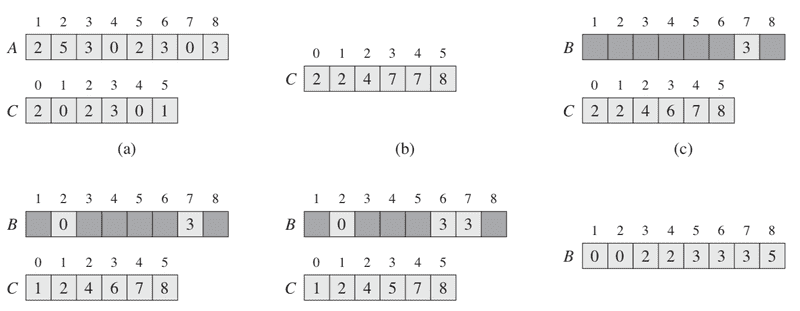
\includegraphics[width=0.7\textwidth]{img/CountS}
\caption{Algoritmo Counting Sort}
\label{fig:CountS}
\end{figure}


		
		Solución \\
		.................
		
		\item Algoritmo Heapsort
		
		Solución \\
		.................

        \item Algoritmo Merge Sort
		
		Solución \\
		.................
		
	    \item Algoritmo Quicksort

		
	\end{enumerate}


\section{Conclusiones}
	
	%\clearpage
	%\bibliographystyle{apalike}
	%\bibliographystyle{IEEEtranN}
	%\bibliography{bibliography}
		
	
\end{document}
